\chapter{Bootproces}

\section{Opstarten}

Het opstartproces van een computer begint wanneer de voeding van
de computer ingeschakeld wordt. Bij het inschakelen controleert de
voeding zijn eigen spanningsniveaus. Wanneer de spanning stabiel is
tussen aanvaardbare waarden wordt een 'Power Good'\index{power good} signaal
gestuurd naar het moederbord. Het duurt typisch tussen 0,1 en 0,5
seconden voor de voeding stabiele stroom kan leveren.

Een halve seconde lijkt niet veel, maar de huidige processoren
voeren in die tijd miljoenen instructies uit. Om te vermijden dat het
systeem onder deze onstabiele omstandigheden zou beginnen opstarten
blijft het moederbord de processor continu resetten zolang er geen power
good signaal ontvangen wordt. Ook wanneer de computer al in gebruik is
verhindert dit mechanisme beschadiging of onzekere resultaten door
slechte stroomtoevoer. Bij problemen met de stroomvoorziening, zoals een
abnormale spanningswijziging op het stroomnet, zal het systeem zichzelf
herstarten omdat de processor weer tijdelijk het reset-signaal ontvangt
wanneer het power good signaal vanuit de voeding wegvalt.

Wanneer het reset-signaal wegvalt kan de processor beginnen
werken. De processor draait nu in kernel mode (d.i.: alle instructies
---ook de gepriviligeerde instructies--- zijn toegelaten) en gebruikt
uit compatibiliteitsoverwegingen \emph{real mode}\index{real mode}
als addresseringsmodus\footnote{Indien je niet meer weet wat \emph{real mode}
is, dan kan je dat best nog eens opzoeken in hoofdstuk 3 van de cursus
Computersystemen}. Maar welke code moet er uitgevoerd worden? Er zijn nog geen
instructies in het werkgeheugen geladen, dus de opstartcode moet elders
gevonden worden.

De oplossing voor dit probleem is om bepaalde adressen in de geheugenruimte niet
mappen op het werkgeheugen maar op iets anders. Dit noemt men \emph{memory mapped I/O}. Figuur~\ref{memorymapped}
toont de layout van de x86-geheugenruimte en welke stukken waarop gemapped worden.
Het rode stuk in de tekening is het stuk van de geheugenruimte waar de processor
de opstartcode verwacht. Concreet begint de processor instructies uit te voeren
vanaf adres 0xFFFFFFF0 (merk op dat dit adres binnen het rode stuk valt). Wanneer
de processor het geheugenadres 0xFFFFFFF0 opvraagt aan de geheugen controller, zal
die echter geen bytes vanuit het werkgeheugen halen, maar zal die de data halen uit
een ROM-chip op het moederbord. Deze ROM-chip bevat dan het opstartprogramma.

\begin{figure}
\centering
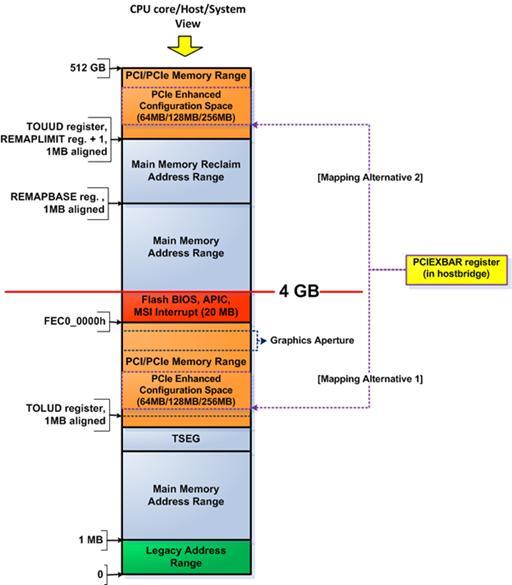
\includegraphics[scale=.75]{images/iomappedmemory.png}
\caption{De x86 memory layout. Leer deze grafiek alsjeblieft niet vanbuiten!}
\label{memorymapped}
\end{figure}

\section{Unified Extensible Firmware Interface}

Moderne systemen volgen de \emph{Unified Extensible Firmware Interface}-specificatie
(\emph{UEFI})\index{UEFI} om de computer verder op te starten. De UEFI-standaard zorgt voor afspraken omtrent een zogenaamde
\emph{pre-boot execution environment} die er voor zorgt dat de hardware ge\"initialiseerd
wordt en het besturingssysteem ingeladen wordt. Implementaties van deze standaard zijn in essentie een
mini-besturingssysteem die een aantal basisfunctionaliteiten aanbieden (zoals bijvoorbeeld
het starten van het hoofdbesturingssysteem).

De belangrijkste eigenschappen die de UEFI-standaard voorziet, zijn:

\begin{itemize}
\item \textbf{Ondersteuning voor grote schijven} De voorganger van UEFI ---{} het Basic Input/Output System (BIOS)\index{basic input/output system} ---{} bood maar ondersteuning voor harde schijven tot 2TB. De UEFI-standaard verhoogt deze limiet tot 8ZB (d.i. 8 miljard terabyte).
\item \textbf{CPU-onafhankelijke architectuur} De UEFI-specificatie is zo opgesteld dat de services die worden aangeboden niet processor-specifiek zijn. Er zijn dan ook UEFI-implementaties voor de x86-, x86-64-, ARM-, ARM64-, en Itanium-processoren.
\item \textbf{CPU-onafhankelijke stuurprogramma's} EFI Byte Code (EBC) is een processor-onafhankelijke machinetaal die een beetje vergelijkbaar is met Java bytecode\footnote{https://en.wikipedia.org/wiki/Java\_bytecode} of Common Intermediate Language\footnote{https://en.wikipedia.org/wiki/Common\_Intermediate\_Language}. Een UEFI-implementatie kan dan een vertolker bevatten om die EBC uit te voeren. Zo moet een auteur van een stuurprogramma slechts \'e\'en versie van het stuurprogramma schrijven (in EBC), dat dan op alle processorarchitecturen waar UEFI op ondersteund wordt kan gebruikt worden.\footnote{In praktijk gaan hardwareontwerpers echter nog vaak processor-specifieke drivers voorzien omdat die vaak een stuk sneller zijn dan de EBC-varianten.}
\item \textbf{Modulair ontwerp} De UEFI-standaard voorziet een aantal mogelijke diensten die kunnen aangeboden worden, maar niet alle diensten \emph{moeten} aangeboden worden.
\item \textbf{Flexibele pre-OS omgeving} Hardwareverkopers krijgen de vrijheid om te kiezen hoe de layout van de pre-OS-omgeving eruit ziet en welke features ze willen ondersteunen. Verder kunnen gebruikers ook nog UEFI-applicaties installeren die dan uitgevoerd worden voordat het besturingssysteem opgestart is. Voorbeelden van zulke applicaties zijn bijvoorbeeld \emph{boot loaders} die dienen om de gebruiker te laten kiezen tussen verschillende besturingssystemen die ge\"installeerd zijn.
\item \textbf{Backward en forward compatibiliteit} UEFI voorziet een compatibiliteits-module om achterwaarts compatibel te zijn met besturingssystemen die geschreven zijn voor de BIOS-voorganger. Verder proberen de auteurs van UEFI ook voorwaarts compatibel te zijn, zodat nieuwe technologie\"en naadloos kunnen gebruikt worden op reeds bestaande UEFI-systemen.
\end{itemize}

UEFI voorziet \emph{boot services} en \emph{runtime services}. Boot services zijn enkel beschikbaar voordat het besturingssysteem opgestart is. Zo zijn er services om uitvoer op het scherm te tonen, communicatie met hardware te verzorgen, enz. De runtime services blijven beschikbaar, ook wanneer het besturingssysteem operationeel is. Zo kan het besturingssysteem bijvoorbeeld de datum en de tijd opvragen, of kan het kleine stukjes data opslaan in de chip waar de UEFI-implementatie in staat.\footnote{Dit is ook de reden waarom je bij het vervangen van een harde schijf je Windows 10 productsleutel niet opnieuw moet ingeven; de Windows 10-setup gaat automatisch je productsleutel opslaan in de UEFI-chip, zodat je die later niet meer opnieuw moet ingeven.}

\begin{figure}
\centering
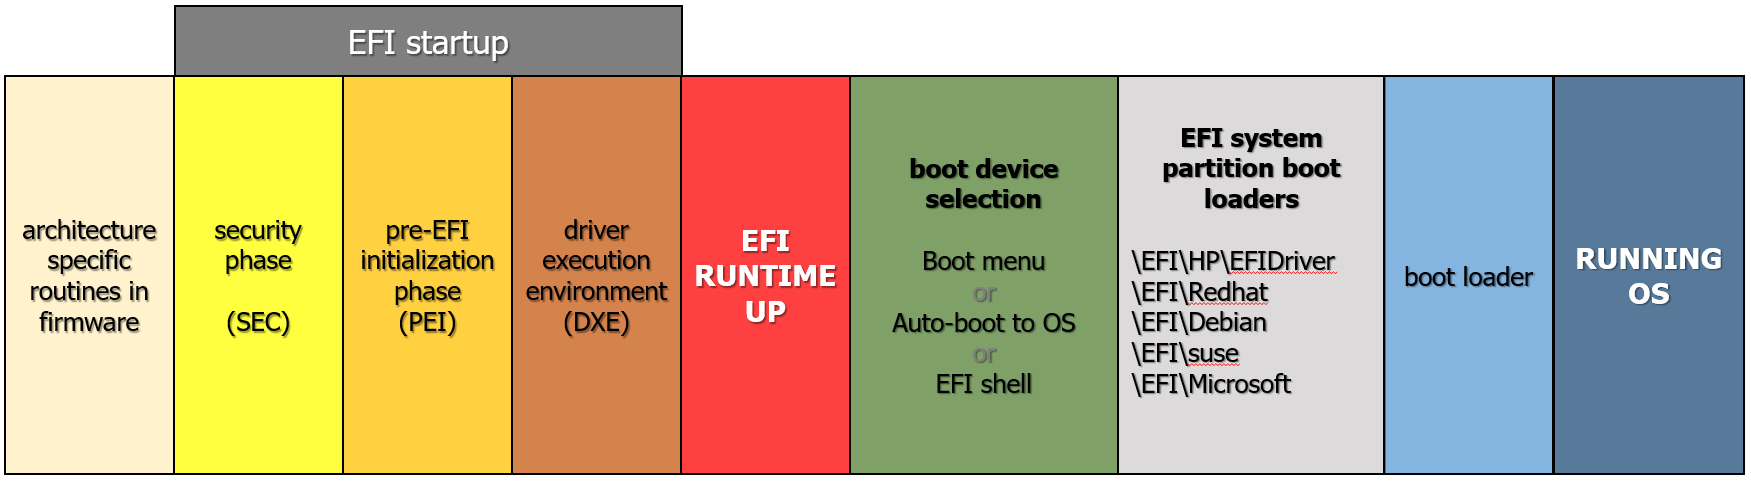
\includegraphics[scale=.25]{images/uefisartup.png}
\caption{Het UEFI boot-proces}
\label{uefiboot}
\end{figure}

De UEFI-specificatie voorziet een aantal fases tijdens het opstarten, zoals weergegeven in figuur~\ref{uefiboot}.
De \emph{security phase} (SEC) controleert dat de code van de UEFI-implementatie correct is en niet aangepast
werd door een potenti\"ele aanvaller. Als een hacker de opstartcode zou kunnen aanpassen, dan zou dat vanzelfsprekend
een zeer groot beveiligingsprobleem zijn. Het doel van de \emph{pre-EFI initialization phase} (PEI) is het opzetten van
een stuk werkgeheugen die de opstartcode kan gebruiken om bijvoorbeeld de UEFI-applicaties in te laden. De \emph{driver
execution phase} (DXE) doet dan het meeste werk wat betreft de initialisatie van het systeem. Hier worden de boot- en
runtime service opgezet, worden hardware-componenten ge\"initialiseerd (harde schijf, netwerk, ...), en worden er abstracties
gecre\"erd voor onder andere de verschillende boot devices. 

De UEFI-specificatie is nogal vaag over wat er precies moet gebeuren wanneer de machine opgestart wordt. Typisch zullen
UEFI-implementaties tijdens de DXE-fase beginnen met het oplijsten van alle beschikbare stukken hardware en controleren
of die correct werken. Het geheel van deze tests wordt \emph{Power-On Self Test}\index{power-on self test} genoemd, of
kortweg \emph{POST}. Op sommige systemen kan je kiezen om deze POST aan te passen of grotendeels over te slaan. Het
voordeel is dan dat je computer sneller opstart, maar je zal een aantal opties (zoals het opstarten vanaf een USB stick)
niet meer kunnen gebruiken.

Als de initialisatie succesvol voltooid is zal de UEFI-code beginnen met
het laden van het besturingssysteem. Dit staat typisch op een
secundair opslagapparaat. Wanneer een computersysteem meerdere van
dergelijke opslagapparaten bevat moet de gebruiker aangeven vanop
welk apparaat een besturingssysteem geladen moet worden. Het
besturingssysteem kan op een harde schijf staan, maar het zou ook op
een CD-ROM, diskette of USB-opslagapparaat. In welke volgorde op alle
aanwezige apparaten naar een besturingssysteem gezocht moet worden
staat in de zogenaamde \emph{opstartvolgorde} of
\emph{boot sequence}\index{boot sequence}. De gebruiker kan deze opstartvolgorde naar eigen keuze aanpassen.

\section{Schijven en partities}

Als in de opstartvolgorde verwezen wordt naar een harde schijf
is de vraag weer hoe we het besturingssysteem terugvinden. De schijf kan in verschillende stukken
opgedeeld zijn (zogenaamde \emph{partities})\index{partitie}, en op eender welke partitie kan het besturingssysteem staan.
Het is aan de gebruiker om via de UEFI-gebruikersinterface de juiste partitie te kiezen.

Het opsplitsen van een schijf in verschillende stukken heeft praktisch nut:
\begin{itemize}
\item Er kan een partitie worden gemaakt voor de bestanden van het besturingssysteem, die enkel bestaat uit de snelste sporen van de schijf.\footnote{\textbf{vraag:} \emph{Welke sporen op de harde schijf zijn de snelste? Denk aan de `zone bit recording'-technologie die in Computersystemen besproken is.}}
\item Het systeem is iets robuuster: je kan makkelijker de beveiliging per partitie instellen, als een programma vanwege een bug de schijf helemaal vult dan heb je daar maar last van op \'e\'en partitie, ...
\item Verschillende partities kunnen verschillende besturingssystemen bevatten (dit noemt men een zogenaamde \emph{multiboot}-opstelling)\index{multiboot}.
\item Zorgt voor een duidelijk scheiding tussen bijvoorbeeld het systeem en databestanden.
\item ...
\end{itemize}

Indien de gebruiker op meerdere partities een besturingssysteem ge\"installeerd heeft, dan kan er een
\emph{boot menu}\index{boot menu} gebruikt worden. Het boot menu toont tijdens het opstartproces een lijst van alle
ge\"installeerde besturingssystemen en laat de gebruiker kiezen welke hij wil opstarten. Figuur~\ref{fig:bootloaders}
toont twee voorbeelden van boot menus.

\begin{figure}
\centering
\begin{subfigure}{.5\textwidth}
  \centering
  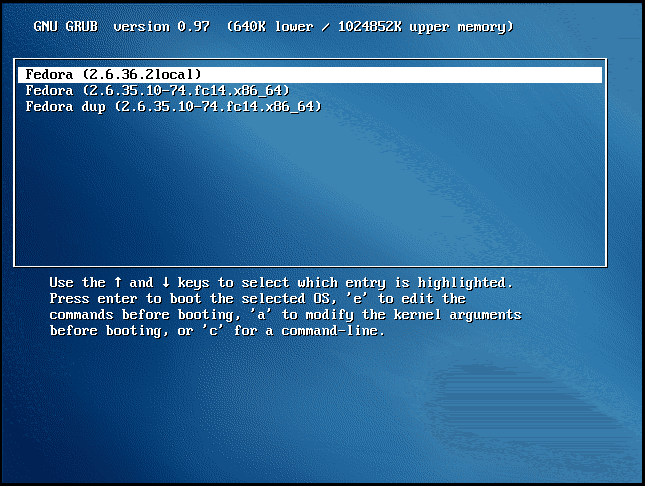
\includegraphics[width=.95\linewidth]{images/grubbl.png}
  \caption{De GRUB boot manager}
  \label{fig:grubnl}
\end{subfigure}%
\begin{subfigure}{.5\textwidth}
  \centering
  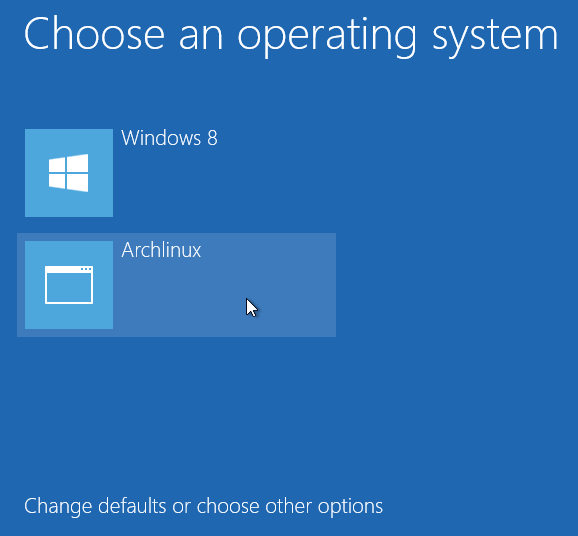
\includegraphics[width=.95\linewidth]{images/wbl.png}
  \caption{De Windows boot manager}
  \label{fig:wbl}
\end{subfigure}
\caption{Twee verschillende UEFI boot managers}
\label{fig:bootloaders}
\end{figure}

Informatie over de partities wordt op de schijf zelf opgeslagen op een gestandardiseerde manier. UEFI ondersteunt de oudere \emph{master boot record}-manier\index{master boot record} (MBR) om partitie-informatie op te slaan, maar deze manier biedt maar ondersteuning voor schijven tot 2TB. Bij voorkeur wordt dan ook het nieuwere \emph{GUID partition table}-systeem\index{GUID partition table} (GPT) gebruikt. GPT biedt ondersteuning voor schijven tot 8ZB (d.i. 8 miljard TB).

Figuur~\ref{fig:gpt-layout} toont de layout van een GPT-schijf. Het eerste blok bevat een \emph{protective master boot record}\index{protective master boot record} voor compatibiliteitsdoeleinden met oudere systemen die geen GPT ondersteunen. Deze protective master boot record is grotendeels leeg, en bevat slechts informatie over \'e\'en partitie die de hele schijf beslaat (of voor schijven groter dan 2TB: zo veel plaats beslaat als mogelijk). Het partitietype staat op \byte{EE} wat betekent dat de partitie in feite een GPT-partitie is. Tools die GPT niet ondersteunen zullen dit partitietype niet herkennen, en zouden normaal gezien de partitie (en dus de schijf) met rust laten.

\begin{figure}
\centering
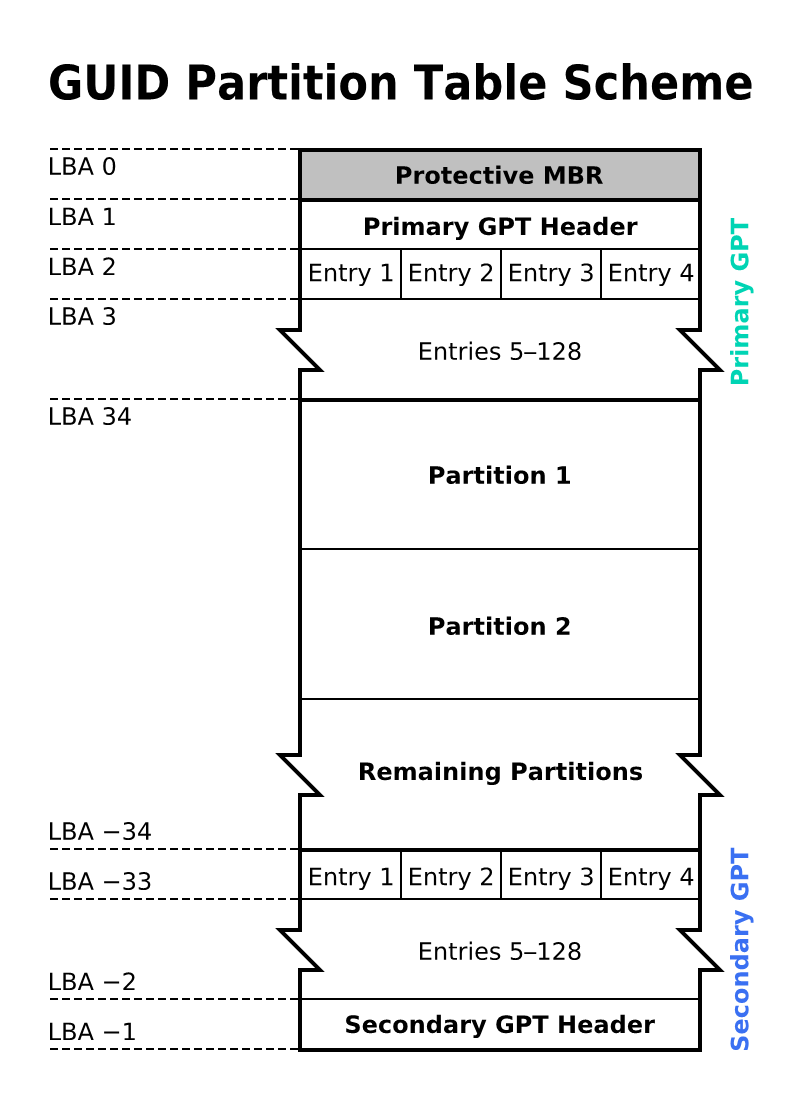
\includegraphics[scale=1]{images/gpt-layout.png}
\caption{De layout van een GPT-schijf}\label{fig:gpt-layout}
\end{figure}

Na de protective MBR staat de primaire GPT header. Deze header bevat informatie over de schijf (grootte, beschikbare sectors, ), een uniek identificatienummer van de schijf, en een wijzer naar een backup-kopie van de header. Deze backup-kopie staat helemaal aan het eind van de schijf en bevat exact dezelfde informatie. Als de primaire header beschadigd raakt, dan kan de backupkopie gebruikt worden om alsnog de partitie-informatie uit te lezen.

Na de primaire GPT header volgt een lijst van \emph{partition entries}.\index{partition entry} Elk van deze entries kan informatie bevatten over \'e\'en partitie. Zo bevat een entry onder andere informatie over het partitietype, een uniek identificatienummer, de start- en eindsector, en de attributen van de partitie (alleen-lezen, verborgen, ...). Ook van de lijst van partition entries wordt een backup op het einde van de schijf bijgehouden.

\begin{figure}
\begin{center}
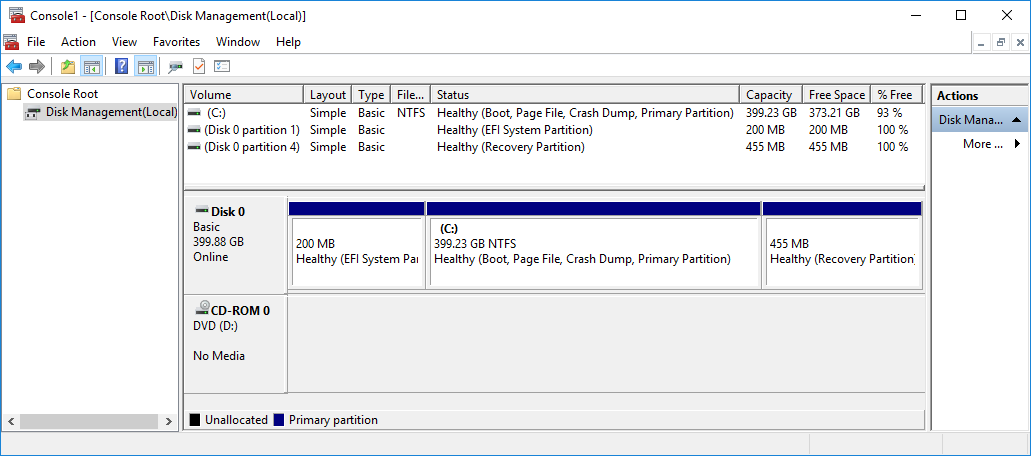
\includegraphics[width=125mm]{images/diskmgr.png}
\end{center}
\caption{Drie GPT-partities}
\label{efisyspart}
\end{figure}

Figuur~\ref{efisyspart} toont een harde schijf met drie partities. De eerste partitie
is van het type \emph{EFI System Partition} en bevat o.a. alle programma's die in de 
UEFI-implementatie uitgevoerd kunnen worden. De tweede partitie bevat in dit geval het
besturingssysteem en is gemarkeerd als \emph{bootable}. Als laatste is er nog een partitie
gedefini\"eerd voor recovery-doeleinden.

Wanneer de UEFI-omgeving opgestart is (d.w.z. de DXE-fase klaar is, zie figuur~\ref{uefiboot}), moet er een
boot device gekozen worden. Hiervoor wordt gebruik gemaakt van een \emph{boot menu}\index{boot menu}-applicatie
die aan de gebruiker vraagt welk besturingssysteem hij wil opstarten. Indien er maar
een besturingssysteem op de computer ge\"installeerd is, is de vraag natuurlijk overbodig
en wordt dit OS direct opgestart. Deze applicatie kan meegeleverd worden door de UEFI-fabrikant, maar kan
ook op de EFI System Partition worden ge\"installeerd bij de installatie van een besturingssysteem op je computer.
Wanneer je bijvoorbeeld Windows installeert, zal de Windows-installatie Microsoft's
boot menu op de EFI System Partition zetten waarmee Windows (en eventueel andere besturingssystemen)
opgestart kan worden.

Eenmaal de gebruiker een besturingssysteem geselecteerd heeft, wordt er een \emph{partition boot loader}\index{partition boot loader}-applicatie opgestart die het besturingssysteem op de geselecteerde partitie zal inladen. Afhankelijk van de gekozen
partitie zal de juiste partition boot loader geselecteerd worden. De taak van de partition boot loader is om op de partitie 
de code te zoeken die het besturingssysteem verder gaat inladen. Kwestie van de zaken wat gecompliceerd te maken, noemen ze deze code
de \emph{boot loader}\index{boot loader}. Zorg dus dat je de termen \emph{boot loader} en \emph{partition boot loader} niet door elkaar
haalt.

De boot loader staat op de partitie van het besturingssysteem en is dus geen deel van de UEFI-implementatie. Als de partitie
bijvoorbeeld een (recente) Windows-installatie bevat, dan zal de boot loader in de eerste sector van de partitie staan\footnote{Indien de eerste sector van de schijf een boot loader bevat, wordt deze sector ook de \emph{partition boot block} of het \emph{partition boot record} genoemd.\index{boot sector}} en het
programma \emph{BOOTMGR} opstarten. BOOTMGR is dan de laatste schakel in het bootproces. Dit programma gaat de feitelijke code van Windows inladen en opstarten. Figuur~\ref{bootsteps} geeft een overzicht van de verschillende stappen in het opstartproces.

\begin{figure}
\begin{center}
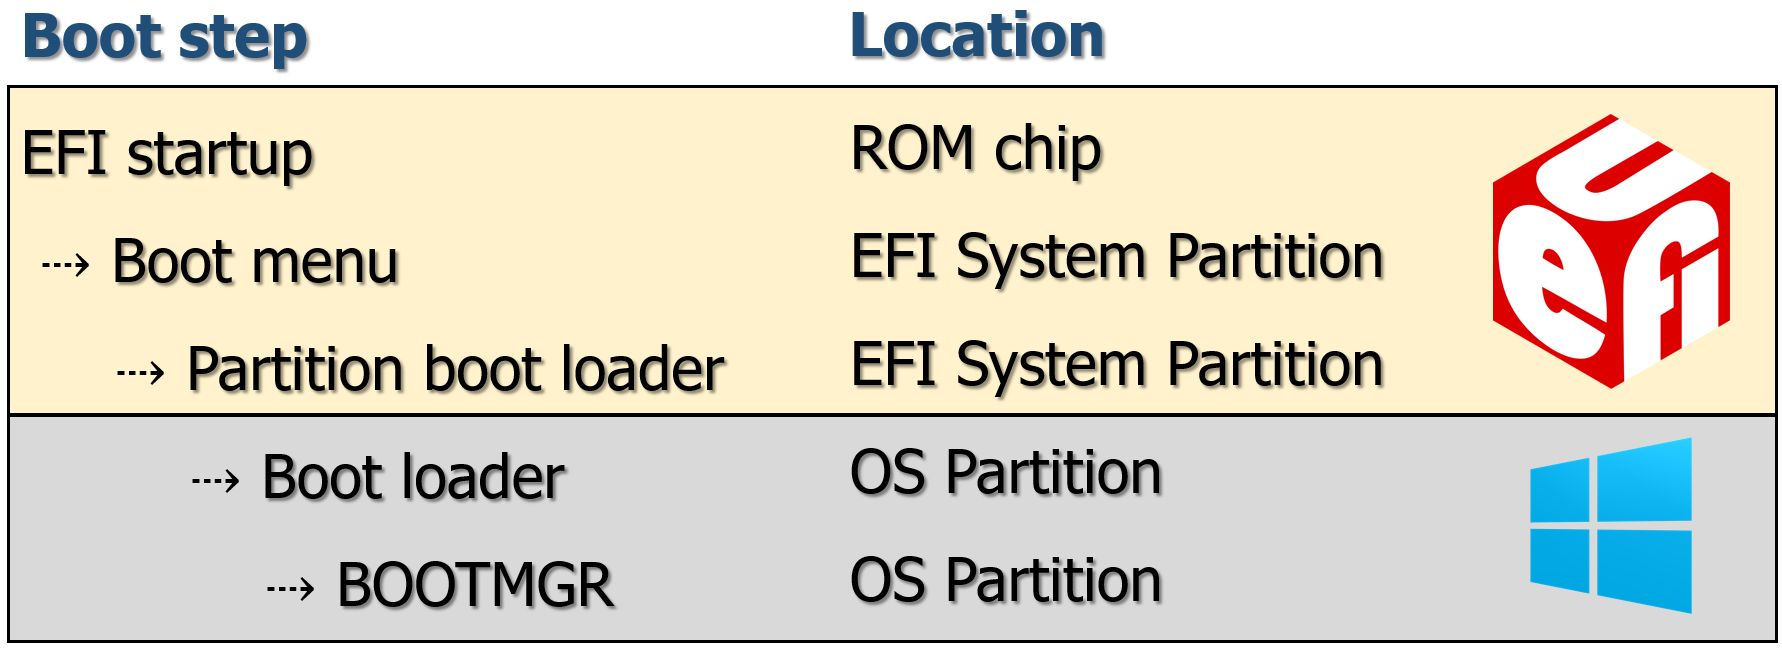
\includegraphics[width=125mm]{images/startupsteps.png}
\end{center}
\caption{De stappen in het opstartproces}
\label{bootsteps}
\end{figure}
